\pagebreak
\setauthorname{Lukas Schachinger}
\chapter{Unity}

\section{Einführung}
Unity (auch bekannt als Unity3D) ist eine Game Engine und \bettergls{ide}{1} zum kreieren von Interaktionsmedien, meißt Video Spielen. \Cite[][A history of the unity game engine]{haas2014history} \\

Die Game Engine wurde in Kopenhagen in 2005 veröffentlicht und ist bekannt für Spiele wie zum Beispiel: \verb+Among Us+, \verb+Monument Valley+, \verb+Pokemon Go+ oder dem Shooter \verb+Escape from Tarkov+. Die Game Engine wurde mit C++ geschrieben, aber ermöglicht den Nutzern mit der zugänglicheren Programmiersprache C\# zu arbeiten. Außerdem bietet die Game Engine die Möglichkeit mit einem Visuellen Editor die Level zu gestalten.

\subsection{Game Objects und Komponenten}
Jedes Game-Object, oder auch Spiel-Objekt in Deutsch, kann eine Vielzahl von Komponenten annehmen. Die nächsten Unterkapitel beschreiben verschiedene solcher Komponenten und stellen diese bildlich dar.

\subsubsection{Das Mesh}
\glqq A mesh consists of triangles arranged in 3D space to create the impression of a solid object. \grqq \Cite[][Anatomy of a Mesh, Unity Documentation]{unitydoc}\\
Ein sogenanntes Mesh definiert das physikalische Objekt. Wie in dem Unity Artikel \verb+Anatomy of a Mesh+ beschrieben ist, besteht das Mesh eines Objektes aus, im 3 Dimensionalen Raum positionierten, Dreiecken die ein solides Objekt darstellen sollen.\\\\
\noindent
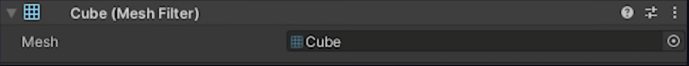
\includegraphics[width=1\linewidth]{chapters/14/Images/Mesh2.png}

\pagebreak

\subsubsection{Der Mesh Renderer}
Der Mesh Renderer ist dafür verantwortlich Materalien und Lichteffekte wie Reflextionen bei einem Objekt darzustellen. Wie in der nächsten Abbildung dargestellt, kann mit dem Mesh Renderer ein Material dem Game-Objekt hinzugefügt werden.\\
\noindent

\begin{figure}[H]
  \centering
  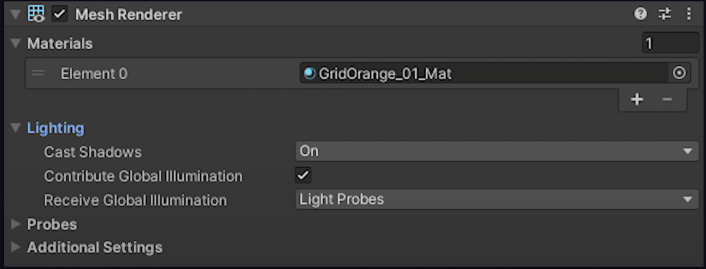
\includegraphics[width=0.7\linewidth]{chapters/14/Images/MeshRenderer.png}
  \caption{Der Mesh Renderer als Komponent.}
  \label{U03}
\end{figure}

\subsubsection{Die Physics Komponenten}
\glqq Wenn ein Rigidbody Komponent zu einem Objekt hinzugefügt wird, dann ist die Bewegung des Objektes unter der Kontrolle von Unitys Physik Engine. Selbst ohne Hinzufügen von Code wird ein Rigidbody-Objekt durch die Schwerkraft nach unten gezogen werden und auf Kollisionen mit einfallenden Objekten reagieren, wenn auch das passende Collider-Komponente vorhanden ist.\grqq \cite[][Rigidbody, Unity Documentation]{unitydocRigidbody} \\

\noindent

\begin{figure}[H]
  \centering
  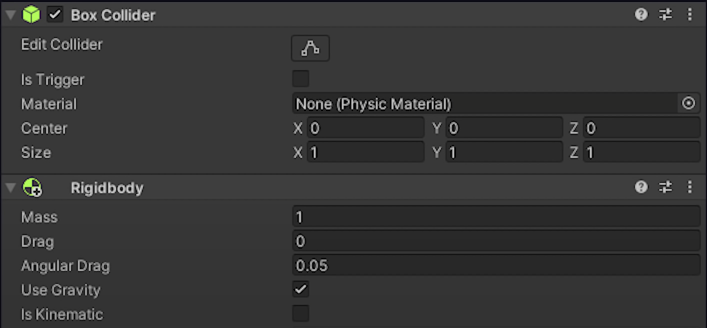
\includegraphics[width=0.7\linewidth]{chapters/14/Images/Physics.png}
  \caption{Die Komponenten für einen Box Collider und Rigidbody.}
  \label{U04}
\end{figure}

\pagebreak
\setauthorname{Lukas Schachinger \& Martin Usta}

\subsubsection{Skript Komponente}
Zudem ist es Möglich einem Game-Objekt ein eigenes Skript als Komponente hinzuzufügen. Mit C\# Code ist es möglich eigene Fähigkeiten oder Attribute dem Objekt zu geben. Zum Beispiel kann eine Variable für \bettergls{hp}{1} angelegt werden. Wenn dieses Game-Objekt dann durch Kontakt mit einem Gegner schaden bekommt, werden Lebenspunkte abgezogen. Wenn diese dann auf Null gelangen, kann mit dem Code das Game-Objekt deaktiviert werden


\subsection{Skybox}\
Eine Skybox ist der Hintergrund unsere Spielewelt. Dabei is Skybox ist ein Würfel, indem sich unsere Spielewelt befindet. Die inneren Seiten des Würfels bilden unseren gesamten Hintergrund.
Zu beachten ist das die Würfelseiten die richtige Textur bekommen. Jede Seite hat seine eigene Koordinate für die vergebene Textur:\\\\

\begin{minipage}{0.4\textwidth}
    \begin{itemize}
        \item +Z für vorne 
        \item -Z für hinten 
        \item +X für links 
        \item -X für rechts
        \item +Y für oben
        \item -Y für unten
    \end{itemize}
  \end{minipage}
  \hfill
  \begin{minipage}{0.6\textwidth}
    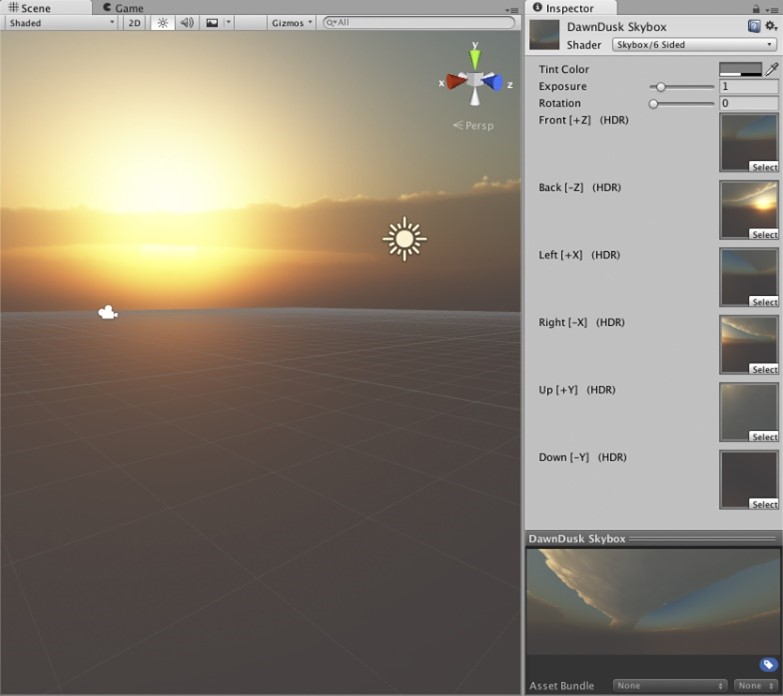
\includegraphics[width=\linewidth]{chapters/14/Images/Skybox.png}
  \end{minipage}

\pagebreak
\subsection{Animation}

Beim Animieren geht es darum, dem Nutzer eine scheinbare Bewegung des Spielobjekts zu vermitteln. Dabei werden die beweglichen Abläufe eines Spielobjekts erstellt und aufgenommen. Hierbei werden die Koordinaten bestimmter Körperelemente in Keyframes festgehalten. Diese können dann auf einer Zeitachse platziert werden. Dadurch wird ein Keyframe mit den gespeicherten Koordinaten zum entsprechenden Zeitpunkt aufgerufen, um eine Bewegung zu simulieren. Jede Münze besitzt diese Animationskomente.

\begin{figure}[H]
  \centering
  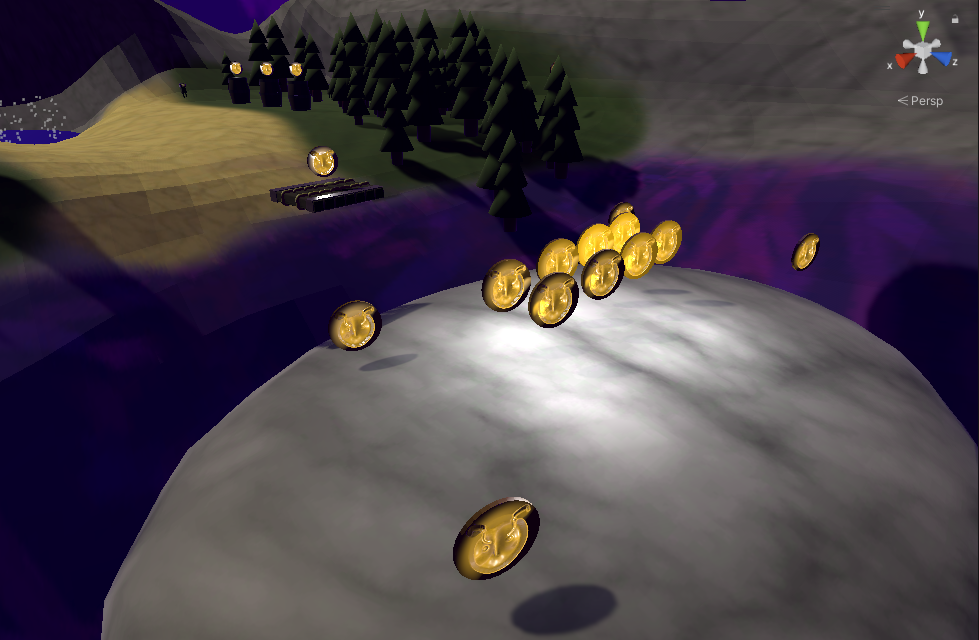
\includegraphics[width=0.5\linewidth]{chapters/14/Images/Animation.png}
  \caption{Eine Abbildung der drehenden Münzen.}
  \label{U06}
\end{figure}

\subsection{Partikel des Portals}

Die Partikel des Portals sind mehrere Game-Objekte die den Partikel Komponenten haben. Dieser musste nur in der Größe und Rotation angepasst werden. Dem Partikel System mussten die Einstellungen und das Material angepasst werden um diesen Effekt zu bekommen.

\begin{figure}[H]
  \centering
  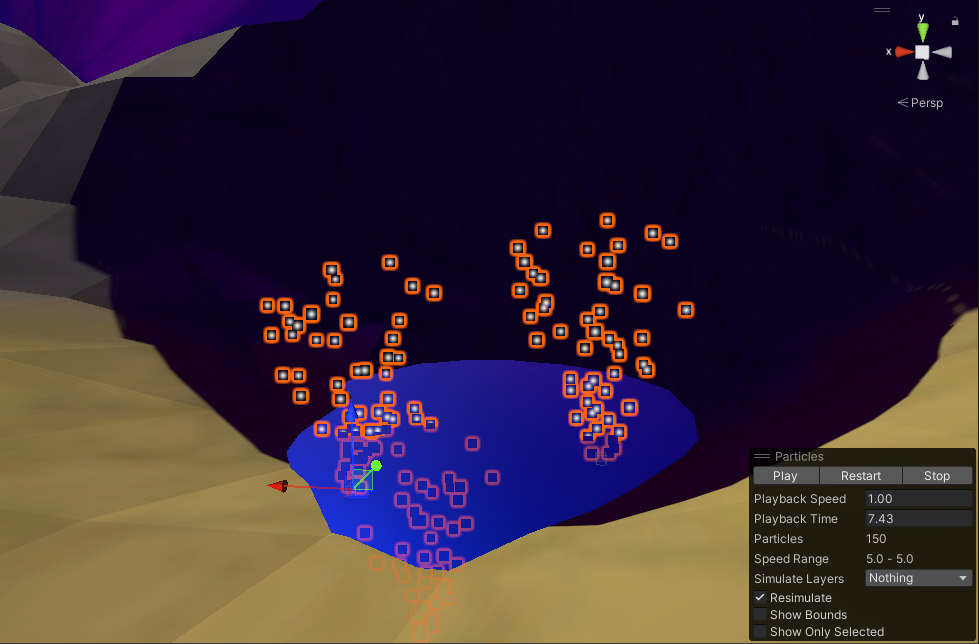
\includegraphics[width=0.5\linewidth]{chapters/14/Images/Partikel.png}
  \caption{Eine Abbildung der Partikel des Portals.}
  \label{U07}
\end{figure}